\documentclass[1p]{elsarticle_modified}
%\bibliographystyle{elsarticle-num}

%\usepackage[colorlinks]{hyperref}
%\usepackage{abbrmath_seonhwa} %\Abb, \Ascr, \Acal ,\Abf, \Afrak
\usepackage{amsfonts}
\usepackage{amssymb}
\usepackage{amsmath}
\usepackage{amsthm}
\usepackage{scalefnt}
\usepackage{amsbsy}
\usepackage{kotex}
\usepackage{caption}
\usepackage{subfig}
\usepackage{color}
\usepackage{graphicx}
\usepackage{xcolor} %% white, black, red, green, blue, cyan, magenta, yellow
\usepackage{float}
\usepackage{setspace}
\usepackage{hyperref}

\usepackage{tikz}
\usetikzlibrary{arrows}

\usepackage{multirow}
\usepackage{array} % fixed length table
\usepackage{hhline}

%%%%%%%%%%%%%%%%%%%%%
\makeatletter
\renewcommand*\env@matrix[1][\arraystretch]{%
	\edef\arraystretch{#1}%
	\hskip -\arraycolsep
	\let\@ifnextchar\new@ifnextchar
	\array{*\c@MaxMatrixCols c}}
\makeatother %https://tex.stackexchange.com/questions/14071/how-can-i-increase-the-line-spacing-in-a-matrix
%%%%%%%%%%%%%%%

\usepackage[normalem]{ulem}

\newcommand{\msout}[1]{\ifmmode\text{\sout{\ensuremath{#1}}}\else\sout{#1}\fi}
%SOURCE: \msout is \stkout macro in https://tex.stackexchange.com/questions/20609/strikeout-in-math-mode

\newcommand{\cancel}[1]{
	\ifmmode
	{\color{red}\msout{#1}}
	\else
	{\color{red}\sout{#1}}
	\fi
}

\newcommand{\add}[1]{
	{\color{blue}\uwave{#1}}
}

\newcommand{\replace}[2]{
	\ifmmode
	{\color{red}\msout{#1}}{\color{blue}\uwave{#2}}
	\else
	{\color{red}\sout{#1}}{\color{blue}\uwave{#2}}
	\fi
}

\newcommand{\Sol}{\mathcal{S}} %segment
\newcommand{\D}{D} %diagram
\newcommand{\A}{\mathcal{A}} %arc


%%%%%%%%%%%%%%%%%%%%%%%%%%%%%5 test

\def\sl{\operatorname{\textup{SL}}(2,\Cbb)}
\def\psl{\operatorname{\textup{PSL}}(2,\Cbb)}
\def\quan{\mkern 1mu \triangleright \mkern 1mu}

\theoremstyle{definition}
\newtheorem{thm}{Theorem}[section]
\newtheorem{prop}[thm]{Proposition}
\newtheorem{lem}[thm]{Lemma}
\newtheorem{ques}[thm]{Question}
\newtheorem{cor}[thm]{Corollary}
\newtheorem{defn}[thm]{Definition}
\newtheorem{exam}[thm]{Example}
\newtheorem{rmk}[thm]{Remark}
\newtheorem{alg}[thm]{Algorithm}

\newcommand{\I}{\sqrt{-1}}
\begin{document}

%\begin{frontmatter}
%
%\title{Boundary parabolic representations of knots up to 8 crossings}
%
%%% Group authors per affiliation:
%\author{Yunhi Cho} 
%\address{Department of Mathematics, University of Seoul, Seoul, Korea}
%\ead{yhcho@uos.ac.kr}
%
%
%\author{Seonhwa Kim} %\fnref{s_kim}}
%\address{Center for Geometry and Physics, Institute for Basic Science, Pohang, 37673, Korea}
%\ead{ryeona17@ibs.re.kr}
%
%\author{Hyuk Kim}
%\address{Department of Mathematical Sciences, Seoul National University, Seoul 08826, Korea}
%\ead{hyukkim@snu.ac.kr}
%
%\author{Seokbeom Yoon}
%\address{Department of Mathematical Sciences, Seoul National University, Seoul, 08826,  Korea}
%\ead{sbyoon15@snu.ac.kr}
%
%\begin{abstract}
%We find all boundary parabolic representation of knots up to 8 crossings.
%
%\end{abstract}
%\begin{keyword}
%    \MSC[2010] 57M25 
%\end{keyword}
%
%\end{frontmatter}

%\linenumbers
%\tableofcontents
%
\newcommand\colored[1]{\textcolor{white}{\rule[-0.35ex]{0.8em}{1.4ex}}\kern-0.8em\color{red} #1}%
%\newcommand\colored[1]{\textcolor{white}{ #1}\kern-2.17ex	\textcolor{white}{ #1}\kern-1.81ex	\textcolor{white}{ #1}\kern-2.15ex\color{red}#1	}

{\Large $\underline{11a_{290}~(K11a_{290})}$}

\setlength{\tabcolsep}{10pt}
\renewcommand{\arraystretch}{1.6}
\vspace{1cm}\begin{tabular}{m{100pt}>{\centering\arraybackslash}m{274pt}}
\multirow{5}{120pt}{
	\centering
	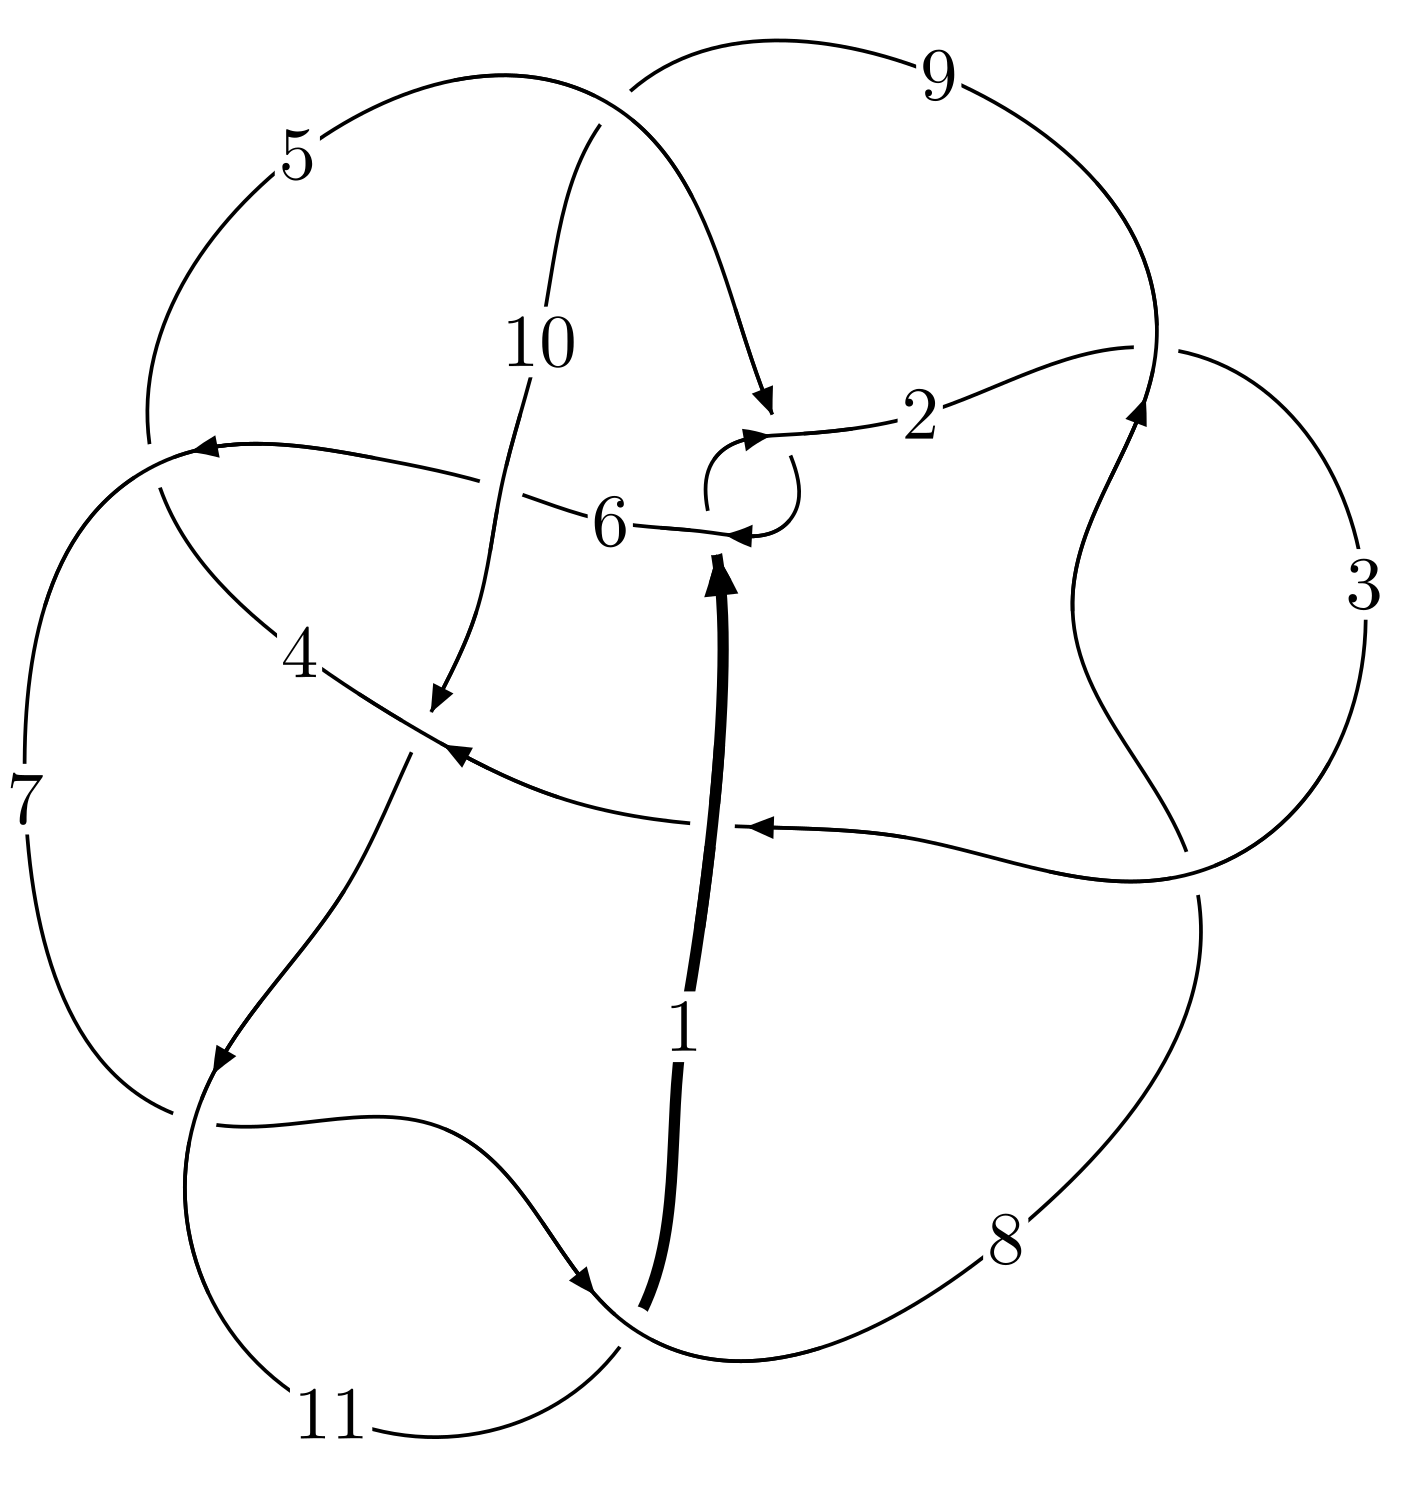
\includegraphics[width=112pt]{../../../GIT/diagram.site/Diagrams/png/539_11a_290.png}\\
\ \ \ A knot diagram\footnotemark}&
\allowdisplaybreaks
\textbf{Linearized knot diagam} \\
\cline{2-2}
 &
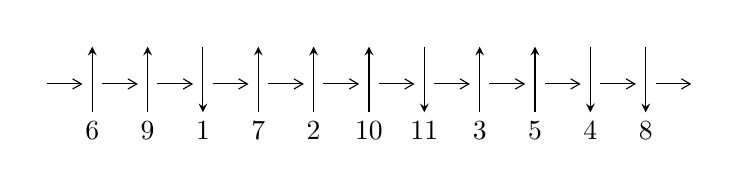
\begin{tikzpicture}[x=20pt, y=17pt]
	% nodes
	\node (C0) at (0, 0) {};
	\node (C1) at (1, 0) {};
	\node (C1U) at (1, +1) {};
	\node (C1D) at (1, -1) {6};

	\node (C2) at (2, 0) {};
	\node (C2U) at (2, +1) {};
	\node (C2D) at (2, -1) {9};

	\node (C3) at (3, 0) {};
	\node (C3U) at (3, +1) {};
	\node (C3D) at (3, -1) {1};

	\node (C4) at (4, 0) {};
	\node (C4U) at (4, +1) {};
	\node (C4D) at (4, -1) {7};

	\node (C5) at (5, 0) {};
	\node (C5U) at (5, +1) {};
	\node (C5D) at (5, -1) {2};

	\node (C6) at (6, 0) {};
	\node (C6U) at (6, +1) {};
	\node (C6D) at (6, -1) {10};

	\node (C7) at (7, 0) {};
	\node (C7U) at (7, +1) {};
	\node (C7D) at (7, -1) {11};

	\node (C8) at (8, 0) {};
	\node (C8U) at (8, +1) {};
	\node (C8D) at (8, -1) {3};

	\node (C9) at (9, 0) {};
	\node (C9U) at (9, +1) {};
	\node (C9D) at (9, -1) {5};

	\node (C10) at (10, 0) {};
	\node (C10U) at (10, +1) {};
	\node (C10D) at (10, -1) {4};

	\node (C11) at (11, 0) {};
	\node (C11U) at (11, +1) {};
	\node (C11D) at (11, -1) {8};
	\node (C12) at (12, 0) {};

	% arrows
	\draw[->,>={angle 60}]
	(C0) edge (C1) (C1) edge (C2) (C2) edge (C3) (C3) edge (C4) (C4) edge (C5) (C5) edge (C6) (C6) edge (C7) (C7) edge (C8) (C8) edge (C9) (C9) edge (C10) (C10) edge (C11) (C11) edge (C12) ;	\draw[->,>=stealth]
	(C1D) edge (C1U) (C2D) edge (C2U) (C3U) edge (C3D) (C4D) edge (C4U) (C5D) edge (C5U) (C6D) edge (C6U) (C7U) edge (C7D) (C8D) edge (C8U) (C9D) edge (C9U) (C10U) edge (C10D) (C11U) edge (C11D) ;
	\end{tikzpicture} \\
\hhline{~~} \\& 
\textbf{Solving Sequence} \\ \cline{2-2} 
 &
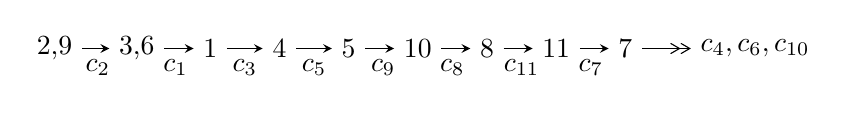
\begin{tikzpicture}[x=25pt, y=7pt]
	% node
	\node (A0) at (-1/8, 0) {2,9};
	\node (A1) at (17/16, 0) {3,6};
	\node (A2) at (17/8, 0) {1};
	\node (A3) at (25/8, 0) {4};
	\node (A4) at (33/8, 0) {5};
	\node (A5) at (41/8, 0) {10};
	\node (A6) at (49/8, 0) {8};
	\node (A7) at (57/8, 0) {11};
	\node (A8) at (65/8, 0) {7};
	\node (C1) at (1/2, -1) {$c_{2}$};
	\node (C2) at (13/8, -1) {$c_{1}$};
	\node (C3) at (21/8, -1) {$c_{3}$};
	\node (C4) at (29/8, -1) {$c_{5}$};
	\node (C5) at (37/8, -1) {$c_{9}$};
	\node (C6) at (45/8, -1) {$c_{8}$};
	\node (C7) at (53/8, -1) {$c_{11}$};
	\node (C8) at (61/8, -1) {$c_{7}$};
	\node (A9) at (10, 0) {$c_{4},c_{6},c_{10}$};

	% edge
	\draw[->,>=stealth]	
	(A0) edge (A1) (A1) edge (A2) (A2) edge (A3) (A3) edge (A4) (A4) edge (A5) (A5) edge (A6) (A6) edge (A7) (A7) edge (A8) ;
	\draw[->>,>={angle 60}]	
	(A8) edge (A9);
\end{tikzpicture} \\ 

\end{tabular} \\

\footnotetext{
The image of knot diagram is generated by the software ``\textbf{Draw programme}" developed by Andrew Bartholomew(\url{http://www.layer8.co.uk/maths/draw/index.htm\#Running-draw}), where we modified some parts for our purpose(\url{https://github.com/CATsTAILs/LinksPainter}).
}\phantom \\ \newline 
\centering \textbf{Ideals for irreducible components\footnotemark of $X_{\text{par}}$} 
 
\begin{align*}
I^u_{1}&=\langle 
-5.37582\times10^{277} u^{85}+1.96137\times10^{278} u^{84}+\cdots+1.50205\times10^{280} b+1.64826\times10^{280},\\
\phantom{I^u_{1}}&\phantom{= \langle  }-9.79158\times10^{279} u^{85}+4.00194\times10^{280} u^{84}+\cdots+2.71871\times10^{282} a+2.80758\times10^{282},\\
\phantom{I^u_{1}}&\phantom{= \langle  }u^{86}-3 u^{85}+\cdots+1252 u+181\rangle \\
I^u_{2}&=\langle 
2984 u^{15}+8425 u^{14}+\cdots+8374 b-4575,\;-28033 u^{15}-151872 u^{14}+\cdots+159106 a+94137,\\
\phantom{I^u_{2}}&\phantom{= \langle  }u^{16}+4 u^{15}+\cdots-3 u+1\rangle \\
\\
\end{align*}
\raggedright * 2 irreducible components of $\dim_{\mathbb{C}}=0$, with total 102 representations.\\
\footnotetext{All coefficients of polynomials are rational numbers. But the coefficients are sometimes approximated in decimal forms when there is not enough margin.}
\newpage
\renewcommand{\arraystretch}{1}
\centering \section*{I. $I^u_{1}= \langle -5.38\times10^{277} u^{85}+1.96\times10^{278} u^{84}+\cdots+1.50\times10^{280} b+1.65\times10^{280},\;-9.79\times10^{279} u^{85}+4.00\times10^{280} u^{84}+\cdots+2.72\times10^{282} a+2.81\times10^{282},\;u^{86}-3 u^{85}+\cdots+1252 u+181 \rangle$}
\flushleft \textbf{(i) Arc colorings}\\
\begin{tabular}{m{7pt} m{180pt} m{7pt} m{180pt} }
\flushright $a_{2}=$&$\begin{pmatrix}1\\0\end{pmatrix}$ \\
\flushright $a_{9}=$&$\begin{pmatrix}0\\u\end{pmatrix}$ \\
\flushright $a_{3}=$&$\begin{pmatrix}1\\- u^2\end{pmatrix}$ \\
\flushright $a_{6}=$&$\begin{pmatrix}0.00360156 u^{85}-0.0147200 u^{84}+\cdots-21.7698 u-1.03269\\0.00357899 u^{85}-0.0130580 u^{84}+\cdots-9.94894 u-1.09735\end{pmatrix}$ \\
\flushright $a_{1}=$&$\begin{pmatrix}0.0110795 u^{85}-0.00313808 u^{84}+\cdots-9.57734 u+0.460705\\0.0148192 u^{85}-0.0206209 u^{84}+\cdots+24.7475 u+3.74548\end{pmatrix}$ \\
\flushright $a_{4}=$&$\begin{pmatrix}-0.00535817 u^{85}+0.0164595 u^{84}+\cdots+31.0765 u+3.73032\\0.00748731 u^{85}-0.0280075 u^{84}+\cdots-23.3642 u-3.54432\end{pmatrix}$ \\
\flushright $a_{5}=$&$\begin{pmatrix}0.0000225642 u^{85}-0.00166203 u^{84}+\cdots-11.8208 u+0.0646558\\0.00357899 u^{85}-0.0130580 u^{84}+\cdots-9.94894 u-1.09735\end{pmatrix}$ \\
\flushright $a_{10}=$&$\begin{pmatrix}0.00480532 u^{85}-0.00440844 u^{84}+\cdots+41.7070 u+5.30239\\0.00626377 u^{85}-0.0151027 u^{84}+\cdots+1.39732 u+0.676884\end{pmatrix}$ \\
\flushright $a_{8}=$&$\begin{pmatrix}- u\\u^3+u\end{pmatrix}$ \\
\flushright $a_{11}=$&$\begin{pmatrix}0.00788554 u^{85}-0.0135049 u^{84}+\cdots-24.0195 u-1.63228\\0.00703857 u^{85}-0.00686933 u^{84}+\cdots+13.6359 u+2.22777\end{pmatrix}$ \\
\flushright $a_{7}=$&$\begin{pmatrix}-0.00149491 u^{85}-0.0103635 u^{84}+\cdots-63.8971 u-7.88042\\-0.0199005 u^{85}+0.0905386 u^{84}+\cdots+16.1319 u+2.96059\end{pmatrix}$\\ \flushright $a_{7}=$&$\begin{pmatrix}-0.00149491 u^{85}-0.0103635 u^{84}+\cdots-63.8971 u-7.88042\\-0.0199005 u^{85}+0.0905386 u^{84}+\cdots+16.1319 u+2.96059\end{pmatrix}$\\&\end{tabular}
\flushleft \textbf{(ii) Obstruction class $= -1$}\\~\\
\flushleft \textbf{(iii) Cusp Shapes $= 0.0176283 u^{85}+0.178110 u^{84}+\cdots+296.326 u+45.8239$}\\~\\
\newpage\renewcommand{\arraystretch}{1}
\flushleft \textbf{(iv) u-Polynomials at the component}\newline \\
\begin{tabular}{m{50pt}|m{274pt}}
Crossings & \hspace{64pt}u-Polynomials at each crossing \\
\hline $$\begin{aligned}c_{1},c_{5}\end{aligned}$$&$\begin{aligned}
&u^{86}+28 u^{84}+\cdots+558 u+43
\end{aligned}$\\
\hline $$\begin{aligned}c_{2},c_{8}\end{aligned}$$&$\begin{aligned}
&u^{86}-3 u^{85}+\cdots+1252 u+181
\end{aligned}$\\
\hline $$\begin{aligned}c_{3}\end{aligned}$$&$\begin{aligned}
&u^{86}-10 u^{85}+\cdots-377377 u+57122
\end{aligned}$\\
\hline $$\begin{aligned}c_{4}\end{aligned}$$&$\begin{aligned}
&u^{86}+9 u^{85}+\cdots+6249 u+722
\end{aligned}$\\
\hline $$\begin{aligned}c_{6}\end{aligned}$$&$\begin{aligned}
&u^{86}-2 u^{85}+\cdots+31 u+1
\end{aligned}$\\
\hline $$\begin{aligned}c_{7},c_{11}\end{aligned}$$&$\begin{aligned}
&u^{86}-2 u^{85}+\cdots+15 u+1
\end{aligned}$\\
\hline $$\begin{aligned}c_{9}\end{aligned}$$&$\begin{aligned}
&u^{86}+18 u^{84}+\cdots+257661 u+27211
\end{aligned}$\\
\hline $$\begin{aligned}c_{10}\end{aligned}$$&$\begin{aligned}
&u^{86}-2 u^{85}+\cdots-11 u+1
\end{aligned}$\\
\hline
\end{tabular}\\~\\
\newpage\renewcommand{\arraystretch}{1}
\flushleft \textbf{(v) Riley Polynomials at the component}\newline \\
\begin{tabular}{m{50pt}|m{274pt}}
Crossings & \hspace{64pt}Riley Polynomials at each crossing \\
\hline $$\begin{aligned}c_{1},c_{5}\end{aligned}$$&$\begin{aligned}
&y^{86}+56 y^{85}+\cdots+192768 y+1849
\end{aligned}$\\
\hline $$\begin{aligned}c_{2},c_{8}\end{aligned}$$&$\begin{aligned}
&y^{86}+67 y^{85}+\cdots+1561986 y+32761
\end{aligned}$\\
\hline $$\begin{aligned}c_{3}\end{aligned}$$&$\begin{aligned}
&y^{86}-40 y^{85}+\cdots-106949549161 y+3262922884
\end{aligned}$\\
\hline $$\begin{aligned}c_{4}\end{aligned}$$&$\begin{aligned}
&y^{86}+21 y^{85}+\cdots+18203155 y+521284
\end{aligned}$\\
\hline $$\begin{aligned}c_{6}\end{aligned}$$&$\begin{aligned}
&y^{86}+2 y^{85}+\cdots-173 y+1
\end{aligned}$\\
\hline $$\begin{aligned}c_{7},c_{11}\end{aligned}$$&$\begin{aligned}
&y^{86}-70 y^{85}+\cdots+163 y+1
\end{aligned}$\\
\hline $$\begin{aligned}c_{9}\end{aligned}$$&$\begin{aligned}
&y^{86}+36 y^{85}+\cdots-1107389665 y+740438521
\end{aligned}$\\
\hline $$\begin{aligned}c_{10}\end{aligned}$$&$\begin{aligned}
&y^{86}-18 y^{85}+\cdots-43 y+1
\end{aligned}$\\
\hline
\end{tabular}\\~\\
\newpage\flushleft \textbf{(vi) Complex Volumes and Cusp Shapes}
$$\begin{array}{c|c|c}  
\text{Solutions to }I^u_{1}& \I (\text{vol} + \sqrt{-1}CS) & \text{Cusp shape}\\
 \hline 
\begin{aligned}
u &= \phantom{-}0.273563 + 0.969299 I \\
a &= -0.558541 - 0.791320 I \\
b &= -0.750237 - 0.353855 I\end{aligned}
 & -1.75556 + 2.96398 I & \phantom{-0.000000 } 0 \\ \hline\begin{aligned}
u &= \phantom{-}0.273563 - 0.969299 I \\
a &= -0.558541 + 0.791320 I \\
b &= -0.750237 + 0.353855 I\end{aligned}
 & -1.75556 - 2.96398 I & \phantom{-0.000000 } 0 \\ \hline\begin{aligned}
u &= -0.791405 + 0.487265 I \\
a &= -1.249760 + 0.001637 I \\
b &= \phantom{-}0.176471 - 0.796902 I\end{aligned}
 & -2.76919 + 0.86190 I & \phantom{-0.000000 } 0 \\ \hline\begin{aligned}
u &= -0.791405 - 0.487265 I \\
a &= -1.249760 - 0.001637 I \\
b &= \phantom{-}0.176471 + 0.796902 I\end{aligned}
 & -2.76919 - 0.86190 I & \phantom{-0.000000 } 0 \\ \hline\begin{aligned}
u &= \phantom{-}1.058500 + 0.166799 I \\
a &= \phantom{-}0.195269 - 0.257088 I \\
b &= -0.384724 - 1.167240 I\end{aligned}
 & -0.44655 + 6.40335 I & \phantom{-0.000000 } 0 \\ \hline\begin{aligned}
u &= \phantom{-}1.058500 - 0.166799 I \\
a &= \phantom{-}0.195269 + 0.257088 I \\
b &= -0.384724 + 1.167240 I\end{aligned}
 & -0.44655 - 6.40335 I & \phantom{-0.000000 } 0 \\ \hline\begin{aligned}
u &= \phantom{-}0.433257 + 0.809408 I \\
a &= -0.481754 - 0.210140 I \\
b &= -0.184332 + 0.437485 I\end{aligned}
 & \phantom{-}0.18140 + 1.93771 I & \phantom{-0.000000 } 0 \\ \hline\begin{aligned}
u &= \phantom{-}0.433257 - 0.809408 I \\
a &= -0.481754 + 0.210140 I \\
b &= -0.184332 - 0.437485 I\end{aligned}
 & \phantom{-}0.18140 - 1.93771 I & \phantom{-0.000000 } 0 \\ \hline\begin{aligned}
u &= \phantom{-}0.822552 + 0.231435 I \\
a &= \phantom{-}0.584539 + 0.759190 I \\
b &= -0.725573 + 0.219124 I\end{aligned}
 & -1.52512 + 6.90858 I & \phantom{-0.000000 } 0 \\ \hline\begin{aligned}
u &= \phantom{-}0.822552 - 0.231435 I \\
a &= \phantom{-}0.584539 - 0.759190 I \\
b &= -0.725573 - 0.219124 I\end{aligned}
 & -1.52512 - 6.90858 I & \phantom{-0.000000 } 0\\
 \hline 
 \end{array}$$\newpage$$\begin{array}{c|c|c}  
\text{Solutions to }I^u_{1}& \I (\text{vol} + \sqrt{-1}CS) & \text{Cusp shape}\\
 \hline 
\begin{aligned}
u &= -0.054741 + 1.153840 I \\
a &= -0.24301 + 2.56854 I \\
b &= -0.119574 + 1.052110 I\end{aligned}
 & -1.32630 - 3.41399 I & \phantom{-0.000000 } 0 \\ \hline\begin{aligned}
u &= -0.054741 - 1.153840 I \\
a &= -0.24301 - 2.56854 I \\
b &= -0.119574 - 1.052110 I\end{aligned}
 & -1.32630 + 3.41399 I & \phantom{-0.000000 } 0 \\ \hline\begin{aligned}
u &= \phantom{-}0.079218 + 1.178320 I \\
a &= -0.012899 - 0.520620 I \\
b &= -0.729471 - 0.142215 I\end{aligned}
 & -2.46468 + 1.92737 I & \phantom{-0.000000 } 0 \\ \hline\begin{aligned}
u &= \phantom{-}0.079218 - 1.178320 I \\
a &= -0.012899 + 0.520620 I \\
b &= -0.729471 + 0.142215 I\end{aligned}
 & -2.46468 - 1.92737 I & \phantom{-0.000000 } 0 \\ \hline\begin{aligned}
u &= -0.526037 + 1.072220 I \\
a &= -0.072054 + 0.352626 I \\
b &= -0.200801 - 0.661210 I\end{aligned}
 & -4.76421 - 5.78091 I & \phantom{-0.000000 } 0 \\ \hline\begin{aligned}
u &= -0.526037 - 1.072220 I \\
a &= -0.072054 - 0.352626 I \\
b &= -0.200801 + 0.661210 I\end{aligned}
 & -4.76421 + 5.78091 I & \phantom{-0.000000 } 0 \\ \hline\begin{aligned}
u &= -0.796875 + 0.085423 I \\
a &= -0.340912 - 0.000196 I \\
b &= \phantom{-}0.088188 + 1.153450 I\end{aligned}
 & -2.78970 + 1.91473 I & \phantom{-0.000000 } 0. - 3.13596 I \\ \hline\begin{aligned}
u &= -0.796875 - 0.085423 I \\
a &= -0.340912 + 0.000196 I \\
b &= \phantom{-}0.088188 - 1.153450 I\end{aligned}
 & -2.78970 - 1.91473 I & \phantom{-0.000000 -}0. + 3.13596 I \\ \hline\begin{aligned}
u &= \phantom{-}0.674546 + 0.412385 I \\
a &= -1.71045 - 0.61869 I \\
b &= \phantom{-}0.414687 - 0.836442 I\end{aligned}
 & -3.09982 - 3.89257 I & \phantom{-0.000000 -}0. + 7.60203 I \\ \hline\begin{aligned}
u &= \phantom{-}0.674546 - 0.412385 I \\
a &= -1.71045 + 0.61869 I \\
b &= \phantom{-}0.414687 + 0.836442 I\end{aligned}
 & -3.09982 + 3.89257 I & \phantom{-0.000000 } 0. - 7.60203 I\\
 \hline 
 \end{array}$$\newpage$$\begin{array}{c|c|c}  
\text{Solutions to }I^u_{1}& \I (\text{vol} + \sqrt{-1}CS) & \text{Cusp shape}\\
 \hline 
\begin{aligned}
u &= \phantom{-}0.029748 + 1.211970 I \\
a &= -0.776818 - 0.475869 I \\
b &= -1.251790 - 0.400798 I\end{aligned}
 & -1.72544 + 2.47755 I & \phantom{-0.000000 } 0 \\ \hline\begin{aligned}
u &= \phantom{-}0.029748 - 1.211970 I \\
a &= -0.776818 + 0.475869 I \\
b &= -1.251790 + 0.400798 I\end{aligned}
 & -1.72544 - 2.47755 I & \phantom{-0.000000 } 0 \\ \hline\begin{aligned}
u &= -0.714002 + 0.312630 I \\
a &= -0.466193 - 0.747453 I \\
b &= \phantom{-}0.472121 - 1.150990 I\end{aligned}
 & -2.08518 - 4.50257 I & \phantom{-}1.84178 + 8.26392 I \\ \hline\begin{aligned}
u &= -0.714002 - 0.312630 I \\
a &= -0.466193 + 0.747453 I \\
b &= \phantom{-}0.472121 + 1.150990 I\end{aligned}
 & -2.08518 + 4.50257 I & \phantom{-}1.84178 - 8.26392 I \\ \hline\begin{aligned}
u &= -0.159848 + 1.234050 I \\
a &= \phantom{-}0.529862 - 0.023389 I \\
b &= \phantom{-}1.371900 + 0.103900 I\end{aligned}
 & -1.05879 - 4.77375 I & \phantom{-0.000000 } 0 \\ \hline\begin{aligned}
u &= -0.159848 - 1.234050 I \\
a &= \phantom{-}0.529862 + 0.023389 I \\
b &= \phantom{-}1.371900 - 0.103900 I\end{aligned}
 & -1.05879 + 4.77375 I & \phantom{-0.000000 } 0 \\ \hline\begin{aligned}
u &= \phantom{-}0.538060 + 0.526043 I \\
a &= -0.678151 + 0.085231 I \\
b &= \phantom{-}0.416327 + 0.832614 I\end{aligned}
 & \phantom{-}0.75640 + 1.97088 I & \phantom{-}6.98873 - 3.30851 I \\ \hline\begin{aligned}
u &= \phantom{-}0.538060 - 0.526043 I \\
a &= -0.678151 - 0.085231 I \\
b &= \phantom{-}0.416327 - 0.832614 I\end{aligned}
 & \phantom{-}0.75640 - 1.97088 I & \phantom{-}6.98873 + 3.30851 I \\ \hline\begin{aligned}
u &= \phantom{-}0.246587 + 1.249730 I \\
a &= \phantom{-}0.32583 - 2.92544 I \\
b &= -0.113725 - 1.064060 I\end{aligned}
 & -5.93474 + 7.14233 I & \phantom{-0.000000 } 0 \\ \hline\begin{aligned}
u &= \phantom{-}0.246587 - 1.249730 I \\
a &= \phantom{-}0.32583 + 2.92544 I \\
b &= -0.113725 + 1.064060 I\end{aligned}
 & -5.93474 - 7.14233 I & \phantom{-0.000000 } 0\\
 \hline 
 \end{array}$$\newpage$$\begin{array}{c|c|c}  
\text{Solutions to }I^u_{1}& \I (\text{vol} + \sqrt{-1}CS) & \text{Cusp shape}\\
 \hline 
\begin{aligned}
u &= -0.714469 + 0.107760 I \\
a &= -0.789250 + 0.825546 I \\
b &= -0.0426813 - 0.1283240 I\end{aligned}
 & -2.61985 + 1.17605 I & \phantom{-}1.036569 - 0.187938 I \\ \hline\begin{aligned}
u &= -0.714469 - 0.107760 I \\
a &= -0.789250 - 0.825546 I \\
b &= -0.0426813 + 0.1283240 I\end{aligned}
 & -2.61985 - 1.17605 I & \phantom{-}1.036569 + 0.187938 I \\ \hline\begin{aligned}
u &= \phantom{-}0.078198 + 1.275430 I \\
a &= \phantom{-}1.13726 - 2.18042 I \\
b &= -0.354521 - 1.348510 I\end{aligned}
 & -10.13010 + 5.46901 I & \phantom{-0.000000 } 0 \\ \hline\begin{aligned}
u &= \phantom{-}0.078198 - 1.275430 I \\
a &= \phantom{-}1.13726 + 2.18042 I \\
b &= -0.354521 + 1.348510 I\end{aligned}
 & -10.13010 - 5.46901 I & \phantom{-0.000000 } 0 \\ \hline\begin{aligned}
u &= -0.176487 + 1.270570 I \\
a &= \phantom{-}0.036238 - 0.305363 I \\
b &= \phantom{-}1.043670 - 0.552437 I\end{aligned}
 & -6.11732 - 3.95002 I & \phantom{-0.000000 } 0 \\ \hline\begin{aligned}
u &= -0.176487 - 1.270570 I \\
a &= \phantom{-}0.036238 + 0.305363 I \\
b &= \phantom{-}1.043670 + 0.552437 I\end{aligned}
 & -6.11732 + 3.95002 I & \phantom{-0.000000 } 0 \\ \hline\begin{aligned}
u &= -0.179144 + 1.277070 I \\
a &= -0.26902 - 1.57349 I \\
b &= \phantom{-}0.83796 - 1.48737 I\end{aligned}
 & -8.41301 - 3.69610 I & \phantom{-0.000000 } 0 \\ \hline\begin{aligned}
u &= -0.179144 - 1.277070 I \\
a &= -0.26902 + 1.57349 I \\
b &= \phantom{-}0.83796 + 1.48737 I\end{aligned}
 & -8.41301 + 3.69610 I & \phantom{-0.000000 } 0 \\ \hline\begin{aligned}
u &= -0.261605 + 1.326890 I \\
a &= -0.44168 - 1.72698 I \\
b &= \phantom{-}0.31957 - 1.56887 I\end{aligned}
 & -7.29801 - 1.70122 I & \phantom{-0.000000 } 0 \\ \hline\begin{aligned}
u &= -0.261605 - 1.326890 I \\
a &= -0.44168 + 1.72698 I \\
b &= \phantom{-}0.31957 + 1.56887 I\end{aligned}
 & -7.29801 + 1.70122 I & \phantom{-0.000000 } 0\\
 \hline 
 \end{array}$$\newpage$$\begin{array}{c|c|c}  
\text{Solutions to }I^u_{1}& \I (\text{vol} + \sqrt{-1}CS) & \text{Cusp shape}\\
 \hline 
\begin{aligned}
u &= -0.378360 + 1.326520 I \\
a &= \phantom{-}0.87070 + 1.64004 I \\
b &= -0.428512 + 1.305690 I\end{aligned}
 & -6.77744 - 6.30203 I & \phantom{-0.000000 } 0 \\ \hline\begin{aligned}
u &= -0.378360 - 1.326520 I \\
a &= \phantom{-}0.87070 - 1.64004 I \\
b &= -0.428512 - 1.305690 I\end{aligned}
 & -6.77744 + 6.30203 I & \phantom{-0.000000 } 0 \\ \hline\begin{aligned}
u &= -1.280750 + 0.519114 I \\
a &= \phantom{-}0.389301 + 0.640771 I \\
b &= -0.414651 + 1.174810 I\end{aligned}
 & -4.46055 - 11.18420 I & \phantom{-0.000000 } 0 \\ \hline\begin{aligned}
u &= -1.280750 - 0.519114 I \\
a &= \phantom{-}0.389301 - 0.640771 I \\
b &= -0.414651 - 1.174810 I\end{aligned}
 & -4.46055 + 11.18420 I & \phantom{-0.000000 } 0 \\ \hline\begin{aligned}
u &= -0.019101 + 1.401050 I \\
a &= -0.23552 + 1.78688 I \\
b &= \phantom{-}0.43425 + 1.53897 I\end{aligned}
 & -12.14740 - 4.74643 I & \phantom{-0.000000 } 0 \\ \hline\begin{aligned}
u &= -0.019101 - 1.401050 I \\
a &= -0.23552 - 1.78688 I \\
b &= \phantom{-}0.43425 - 1.53897 I\end{aligned}
 & -12.14740 + 4.74643 I & \phantom{-0.000000 } 0 \\ \hline\begin{aligned}
u &= -0.148079 + 1.400730 I \\
a &= \phantom{-}1.12074 + 1.42376 I \\
b &= -0.110874 + 1.089880 I\end{aligned}
 & -9.95220 - 0.65712 I & \phantom{-0.000000 } 0 \\ \hline\begin{aligned}
u &= -0.148079 - 1.400730 I \\
a &= \phantom{-}1.12074 - 1.42376 I \\
b &= -0.110874 - 1.089880 I\end{aligned}
 & -9.95220 + 0.65712 I & \phantom{-0.000000 } 0 \\ \hline\begin{aligned}
u &= \phantom{-}0.18402 + 1.40665 I \\
a &= \phantom{-}0.18310 - 1.74200 I \\
b &= -0.62071 - 1.36597 I\end{aligned}
 & -5.12935 + 4.31635 I & \phantom{-0.000000 } 0 \\ \hline\begin{aligned}
u &= \phantom{-}0.18402 - 1.40665 I \\
a &= \phantom{-}0.18310 + 1.74200 I \\
b &= -0.62071 + 1.36597 I\end{aligned}
 & -5.12935 - 4.31635 I & \phantom{-0.000000 } 0\\
 \hline 
 \end{array}$$\newpage$$\begin{array}{c|c|c}  
\text{Solutions to }I^u_{1}& \I (\text{vol} + \sqrt{-1}CS) & \text{Cusp shape}\\
 \hline 
\begin{aligned}
u &= -0.35726 + 1.39065 I \\
a &= \phantom{-}0.0345880 + 0.0824053 I \\
b &= -0.833294 - 0.003827 I\end{aligned}
 & -7.36616 - 3.03836 I & \phantom{-0.000000 } 0 \\ \hline\begin{aligned}
u &= -0.35726 - 1.39065 I \\
a &= \phantom{-}0.0345880 - 0.0824053 I \\
b &= -0.833294 + 0.003827 I\end{aligned}
 & -7.36616 + 3.03836 I & \phantom{-0.000000 } 0 \\ \hline\begin{aligned}
u &= \phantom{-}0.32019 + 1.40690 I \\
a &= \phantom{-}0.394902 + 0.096675 I \\
b &= \phantom{-}1.225800 - 0.072859 I\end{aligned}
 & -6.75829 + 10.98080 I & \phantom{-0.000000 } 0 \\ \hline\begin{aligned}
u &= \phantom{-}0.32019 - 1.40690 I \\
a &= \phantom{-}0.394902 - 0.096675 I \\
b &= \phantom{-}1.225800 + 0.072859 I\end{aligned}
 & -6.75829 - 10.98080 I & \phantom{-0.000000 } 0 \\ \hline\begin{aligned}
u &= -0.27512 + 1.42570 I \\
a &= \phantom{-}0.39471 + 2.11603 I \\
b &= -0.47939 + 1.46461 I\end{aligned}
 & -7.64272 - 8.09055 I & \phantom{-0.000000 } 0 \\ \hline\begin{aligned}
u &= -0.27512 - 1.42570 I \\
a &= \phantom{-}0.39471 - 2.11603 I \\
b &= -0.47939 - 1.46461 I\end{aligned}
 & -7.64272 + 8.09055 I & \phantom{-0.000000 } 0 \\ \hline\begin{aligned}
u &= \phantom{-}0.26743 + 1.43796 I \\
a &= -0.124019 + 0.837964 I \\
b &= -0.585323 + 0.305477 I\end{aligned}
 & -5.18226 - 1.85610 I & \phantom{-0.000000 } 0 \\ \hline\begin{aligned}
u &= \phantom{-}0.26743 - 1.43796 I \\
a &= -0.124019 - 0.837964 I \\
b &= -0.585323 - 0.305477 I\end{aligned}
 & -5.18226 + 1.85610 I & \phantom{-0.000000 } 0 \\ \hline\begin{aligned}
u &= \phantom{-}0.531703 + 0.023026 I \\
a &= -0.668608 + 0.076796 I \\
b &= \phantom{-}0.677470 + 0.043888 I\end{aligned}
 & \phantom{-}1.105700 + 0.002392 I & \phantom{-}9.73011 + 0.07496 I \\ \hline\begin{aligned}
u &= \phantom{-}0.531703 - 0.023026 I \\
a &= -0.668608 - 0.076796 I \\
b &= \phantom{-}0.677470 - 0.043888 I\end{aligned}
 & \phantom{-}1.105700 - 0.002392 I & \phantom{-}9.73011 - 0.07496 I\\
 \hline 
 \end{array}$$\newpage$$\begin{array}{c|c|c}  
\text{Solutions to }I^u_{1}& \I (\text{vol} + \sqrt{-1}CS) & \text{Cusp shape}\\
 \hline 
\begin{aligned}
u &= \phantom{-}0.42393 + 1.40684 I \\
a &= -0.49693 + 1.62111 I \\
b &= \phantom{-}0.60345 + 1.42770 I\end{aligned}
 & -5.44322 + 11.59020 I & \phantom{-0.000000 } 0 \\ \hline\begin{aligned}
u &= \phantom{-}0.42393 - 1.40684 I \\
a &= -0.49693 - 1.62111 I \\
b &= \phantom{-}0.60345 - 1.42770 I\end{aligned}
 & -5.44322 - 11.59020 I & \phantom{-0.000000 } 0 \\ \hline\begin{aligned}
u &= -0.491963 + 0.128609 I \\
a &= \phantom{-}0.55174 + 1.79794 I \\
b &= -0.674909 + 0.297545 I\end{aligned}
 & \phantom{-}2.29978 + 2.36466 I & \phantom{-}8.84869 - 2.14342 I \\ \hline\begin{aligned}
u &= -0.491963 - 0.128609 I \\
a &= \phantom{-}0.55174 - 1.79794 I \\
b &= -0.674909 - 0.297545 I\end{aligned}
 & \phantom{-}2.29978 - 2.36466 I & \phantom{-}8.84869 + 2.14342 I \\ \hline\begin{aligned}
u &= -0.62650 + 1.36361 I \\
a &= -0.39539 - 1.41576 I \\
b &= -0.109699 - 1.037280 I\end{aligned}
 & -3.91481 - 0.17244 I & \phantom{-0.000000 } 0 \\ \hline\begin{aligned}
u &= -0.62650 - 1.36361 I \\
a &= -0.39539 + 1.41576 I \\
b &= -0.109699 + 1.037280 I\end{aligned}
 & -3.91481 + 0.17244 I & \phantom{-0.000000 } 0 \\ \hline\begin{aligned}
u &= \phantom{-}0.00350 + 1.52364 I \\
a &= \phantom{-}0.358278 + 1.317200 I \\
b &= -0.550954 + 1.178570 I\end{aligned}
 & -10.65740 - 1.60329 I & \phantom{-0.000000 } 0 \\ \hline\begin{aligned}
u &= \phantom{-}0.00350 - 1.52364 I \\
a &= \phantom{-}0.358278 - 1.317200 I \\
b &= -0.550954 - 1.178570 I\end{aligned}
 & -10.65740 + 1.60329 I & \phantom{-0.000000 } 0 \\ \hline\begin{aligned}
u &= -0.439430 + 0.147669 I \\
a &= -1.44145 + 1.37928 I \\
b &= -0.363451 - 1.148080 I\end{aligned}
 & -4.80669 + 1.43419 I & -5.07531 - 5.47709 I \\ \hline\begin{aligned}
u &= -0.439430 - 0.147669 I \\
a &= -1.44145 - 1.37928 I \\
b &= -0.363451 + 1.148080 I\end{aligned}
 & -4.80669 - 1.43419 I & -5.07531 + 5.47709 I\\
 \hline 
 \end{array}$$\newpage$$\begin{array}{c|c|c}  
\text{Solutions to }I^u_{1}& \I (\text{vol} + \sqrt{-1}CS) & \text{Cusp shape}\\
 \hline 
\begin{aligned}
u &= -0.086601 + 0.438946 I \\
a &= -1.329560 + 0.007199 I \\
b &= \phantom{-}0.590173 + 0.816881 I\end{aligned}
 & \phantom{-}0.92382 + 2.38456 I & \phantom{-}6.67469 + 4.68387 I \\ \hline\begin{aligned}
u &= -0.086601 - 0.438946 I \\
a &= -1.329560 - 0.007199 I \\
b &= \phantom{-}0.590173 - 0.816881 I\end{aligned}
 & \phantom{-}0.92382 - 2.38456 I & \phantom{-}6.67469 - 4.68387 I \\ \hline\begin{aligned}
u &= -0.47210 + 1.56780 I \\
a &= -0.51576 - 1.61493 I \\
b &= \phantom{-}0.59006 - 1.38905 I\end{aligned}
 & -10.9523 - 17.3442 I & \phantom{-0.000000 } 0 \\ \hline\begin{aligned}
u &= -0.47210 - 1.56780 I \\
a &= -0.51576 + 1.61493 I \\
b &= \phantom{-}0.59006 + 1.38905 I\end{aligned}
 & -10.9523 + 17.3442 I & \phantom{-0.000000 } 0 \\ \hline\begin{aligned}
u &= \phantom{-}0.45071 + 1.62342 I \\
a &= -0.35003 + 1.51866 I \\
b &= \phantom{-}0.30166 + 1.40852 I\end{aligned}
 & -12.3927 + 8.1607 I & \phantom{-0.000000 } 0 \\ \hline\begin{aligned}
u &= \phantom{-}0.45071 - 1.62342 I \\
a &= -0.35003 - 1.51866 I \\
b &= \phantom{-}0.30166 - 1.40852 I\end{aligned}
 & -12.3927 - 8.1607 I & \phantom{-0.000000 } 0 \\ \hline\begin{aligned}
u &= \phantom{-}0.59453 + 1.60446 I \\
a &= \phantom{-}0.62690 - 1.41851 I \\
b &= -0.464293 - 1.266200 I\end{aligned}
 & -11.17030 + 7.76159 I & \phantom{-0.000000 } 0 \\ \hline\begin{aligned}
u &= \phantom{-}0.59453 - 1.60446 I \\
a &= \phantom{-}0.62690 + 1.41851 I \\
b &= -0.464293 + 1.266200 I\end{aligned}
 & -11.17030 - 7.76159 I & \phantom{-0.000000 } 0 \\ \hline\begin{aligned}
u &= -0.102691 + 0.229037 I \\
a &= \phantom{-}0.30517 - 2.13509 I \\
b &= \phantom{-}0.898880 - 0.683918 I\end{aligned}
 & \phantom{-}1.09250 - 2.96405 I & \phantom{-}12.5613 + 9.8421 I \\ \hline\begin{aligned}
u &= -0.102691 - 0.229037 I \\
a &= \phantom{-}0.30517 + 2.13509 I \\
b &= \phantom{-}0.898880 + 0.683918 I\end{aligned}
 & \phantom{-}1.09250 + 2.96405 I & \phantom{-}12.5613 - 9.8421 I\\
 \hline 
 \end{array}$$\newpage$$\begin{array}{c|c|c}  
\text{Solutions to }I^u_{1}& \I (\text{vol} + \sqrt{-1}CS) & \text{Cusp shape}\\
 \hline 
\begin{aligned}
u &= \phantom{-}0.077135 + 0.222987 I \\
a &= \phantom{-}3.84908 + 2.69551 I \\
b &= \phantom{-}0.003349 - 1.290410 I\end{aligned}
 & -6.67412 - 4.74942 I & -4.72582 + 5.55088 I \\ \hline\begin{aligned}
u &= \phantom{-}0.077135 - 0.222987 I \\
a &= \phantom{-}3.84908 - 2.69551 I \\
b &= \phantom{-}0.003349 + 1.290410 I\end{aligned}
 & -6.67412 + 4.74942 I & -4.72582 - 5.55088 I \\ \hline\begin{aligned}
u &= \phantom{-}0.66832 + 1.87320 I \\
a &= \phantom{-}0.324156 - 1.096740 I \\
b &= -0.045174 - 1.060190 I\end{aligned}
 & -4.31969 + 0.37021 I & \phantom{-0.000000 } 0 \\ \hline\begin{aligned}
u &= \phantom{-}0.66832 - 1.87320 I \\
a &= \phantom{-}0.324156 + 1.096740 I \\
b &= -0.045174 + 1.060190 I\end{aligned}
 & -4.31969 - 0.37021 I & \phantom{-0.000000 } 0 \\ \hline\begin{aligned}
u &= \phantom{-}2.79686 + 0.72592 I \\
a &= -0.106036 + 0.931168 I \\
b &= \phantom{-}0.072665 + 1.004210 I\end{aligned}
 & -4.97029 - 0.39838 I & \phantom{-0.000000 } 0 \\ \hline\begin{aligned}
u &= \phantom{-}2.79686 - 0.72592 I \\
a &= -0.106036 - 0.931168 I \\
b &= \phantom{-}0.072665 - 1.004210 I\end{aligned}
 & -4.97029 + 0.39838 I & \phantom{-0.000000 } 0\\
 \hline 
 \end{array}$$\newpage\newpage\renewcommand{\arraystretch}{1}
\centering \section*{II. $I^u_{2}= \langle 2984 u^{15}+8425 u^{14}+\cdots+8374 b-4575,\;-2.80\times10^{4} u^{15}-1.52\times10^{5} u^{14}+\cdots+1.59\times10^{5} a+9.41\times10^{4},\;u^{16}+4 u^{15}+\cdots-3 u+1 \rangle$}
\flushleft \textbf{(i) Arc colorings}\\
\begin{tabular}{m{7pt} m{180pt} m{7pt} m{180pt} }
\flushright $a_{2}=$&$\begin{pmatrix}1\\0\end{pmatrix}$ \\
\flushright $a_{9}=$&$\begin{pmatrix}0\\u\end{pmatrix}$ \\
\flushright $a_{3}=$&$\begin{pmatrix}1\\- u^2\end{pmatrix}$ \\
\flushright $a_{6}=$&$\begin{pmatrix}0.176191 u^{15}+0.954533 u^{14}+\cdots-2.25062 u-0.591662\\-0.356341 u^{15}-1.00609 u^{14}+\cdots-5.13566 u+0.546334\end{pmatrix}$ \\
\flushright $a_{1}=$&$\begin{pmatrix}0.106652 u^{15}+0.802999 u^{14}+\cdots+2.04999 u-0.149856\\-0.339981 u^{15}-1.42823 u^{14}+\cdots+5.00060 u-1.61464\end{pmatrix}$ \\
\flushright $a_{4}=$&$\begin{pmatrix}0.137644 u^{15}+0.420336 u^{14}+\cdots+1.85401 u-0.285571\\-0.808021 u^{15}-3.10940 u^{14}+\cdots-5.07303 u+0.205354\end{pmatrix}$ \\
\flushright $a_{5}=$&$\begin{pmatrix}0.532532 u^{15}+1.96062 u^{14}+\cdots+2.88504 u-1.13800\\-0.356341 u^{15}-1.00609 u^{14}+\cdots-5.13566 u+0.546334\end{pmatrix}$ \\
\flushright $a_{10}=$&$\begin{pmatrix}-0.352928 u^{15}-1.82485 u^{14}+\cdots+1.72757 u-2.98321\\0.444697 u^{15}+1.82824 u^{14}+\cdots+2.80468 u-0.446633\end{pmatrix}$ \\
\flushright $a_{8}=$&$\begin{pmatrix}- u\\u^3+u\end{pmatrix}$ \\
\flushright $a_{11}=$&$\begin{pmatrix}0.763711 u^{15}+3.26176 u^{14}+\cdots+2.51728 u-0.476437\\-0.565849 u^{15}-2.48415 u^{14}+\cdots+5.69879 u-1.45754\end{pmatrix}$ \\
\flushright $a_{7}=$&$\begin{pmatrix}-0.894335 u^{15}-4.06800 u^{14}+\cdots-5.46111 u+1.11283\\-0.471126 u^{15}-1.42425 u^{14}+\cdots-4.53190 u+0.730689\end{pmatrix}$\\ \flushright $a_{7}=$&$\begin{pmatrix}-0.894335 u^{15}-4.06800 u^{14}+\cdots-5.46111 u+1.11283\\-0.471126 u^{15}-1.42425 u^{14}+\cdots-4.53190 u+0.730689\end{pmatrix}$\\&\end{tabular}
\flushleft \textbf{(ii) Obstruction class $= 1$}\\~\\
\flushleft \textbf{(iii) Cusp Shapes $= -\frac{369566}{79553} u^{15}-\frac{2837157}{159106} u^{14}+\cdots-\frac{3511991}{79553} u+\frac{872049}{159106}$}\\~\\
\newpage\renewcommand{\arraystretch}{1}
\flushleft \textbf{(iv) u-Polynomials at the component}\newline \\
\begin{tabular}{m{50pt}|m{274pt}}
Crossings & \hspace{64pt}u-Polynomials at each crossing \\
\hline $$\begin{aligned}c_{1}\end{aligned}$$&$\begin{aligned}
&u^{16}- u^{15}+\cdots+3 u+1
\end{aligned}$\\
\hline $$\begin{aligned}c_{2}\end{aligned}$$&$\begin{aligned}
&u^{16}+4 u^{15}+\cdots-3 u+1
\end{aligned}$\\
\hline $$\begin{aligned}c_{3}\end{aligned}$$&$\begin{aligned}
&u^{16}+3 u^{15}+\cdots-6 u+1
\end{aligned}$\\
\hline $$\begin{aligned}c_{4}\end{aligned}$$&$\begin{aligned}
&u^{16}+2 u^{15}+\cdots- u+1
\end{aligned}$\\
\hline $$\begin{aligned}c_{5}\end{aligned}$$&$\begin{aligned}
&u^{16}+u^{15}+\cdots-3 u+1
\end{aligned}$\\
\hline $$\begin{aligned}c_{6}\end{aligned}$$&$\begin{aligned}
&u^{16}-3 u^{15}+\cdots-2 u+1
\end{aligned}$\\
\hline $$\begin{aligned}c_{7}\end{aligned}$$&$\begin{aligned}
&u^{16}+3 u^{15}+\cdots-4 u+3
\end{aligned}$\\
\hline $$\begin{aligned}c_{8}\end{aligned}$$&$\begin{aligned}
&u^{16}-4 u^{15}+\cdots+3 u+1
\end{aligned}$\\
\hline $$\begin{aligned}c_{9}\end{aligned}$$&$\begin{aligned}
&u^{16}+u^{15}+\cdots-2 u+1
\end{aligned}$\\
\hline $$\begin{aligned}c_{10}\end{aligned}$$&$\begin{aligned}
&u^{16}-3 u^{15}+\cdots+4 u+1
\end{aligned}$\\
\hline $$\begin{aligned}c_{11}\end{aligned}$$&$\begin{aligned}
&u^{16}-3 u^{15}+\cdots+4 u+3
\end{aligned}$\\
\hline
\end{tabular}\\~\\
\newpage\renewcommand{\arraystretch}{1}
\flushleft \textbf{(v) Riley Polynomials at the component}\newline \\
\begin{tabular}{m{50pt}|m{274pt}}
Crossings & \hspace{64pt}Riley Polynomials at each crossing \\
\hline $$\begin{aligned}c_{1},c_{5}\end{aligned}$$&$\begin{aligned}
&y^{16}+7 y^{15}+\cdots+9 y+1
\end{aligned}$\\
\hline $$\begin{aligned}c_{2},c_{8}\end{aligned}$$&$\begin{aligned}
&y^{16}+6 y^{15}+\cdots+11 y+1
\end{aligned}$\\
\hline $$\begin{aligned}c_{3}\end{aligned}$$&$\begin{aligned}
&y^{16}-13 y^{15}+\cdots-34 y+1
\end{aligned}$\\
\hline $$\begin{aligned}c_{4}\end{aligned}$$&$\begin{aligned}
&y^{16}+14 y^{14}+\cdots+9 y+1
\end{aligned}$\\
\hline $$\begin{aligned}c_{6}\end{aligned}$$&$\begin{aligned}
&y^{16}+y^{15}+\cdots-8 y+1
\end{aligned}$\\
\hline $$\begin{aligned}c_{7},c_{11}\end{aligned}$$&$\begin{aligned}
&y^{16}-15 y^{15}+\cdots-52 y+9
\end{aligned}$\\
\hline $$\begin{aligned}c_{9}\end{aligned}$$&$\begin{aligned}
&y^{16}- y^{15}+\cdots+8 y+1
\end{aligned}$\\
\hline $$\begin{aligned}c_{10}\end{aligned}$$&$\begin{aligned}
&y^{16}-11 y^{15}+\cdots+6 y+1
\end{aligned}$\\
\hline
\end{tabular}\\~\\
\newpage\flushleft \textbf{(vi) Complex Volumes and Cusp Shapes}
$$\begin{array}{c|c|c}  
\text{Solutions to }I^u_{2}& \I (\text{vol} + \sqrt{-1}CS) & \text{Cusp shape}\\
 \hline 
\begin{aligned}
u &= -0.378111 + 0.978487 I \\
a &= -0.666529 - 0.994815 I \\
b &= -0.073329 + 0.541610 I\end{aligned}
 & -4.37357 - 6.52510 I & \phantom{-}1.74145 + 8.04405 I \\ \hline\begin{aligned}
u &= -0.378111 - 0.978487 I \\
a &= -0.666529 + 0.994815 I \\
b &= -0.073329 - 0.541610 I\end{aligned}
 & -4.37357 + 6.52510 I & \phantom{-}1.74145 - 8.04405 I \\ \hline\begin{aligned}
u &= -0.018830 + 1.228110 I \\
a &= \phantom{-}0.672213 - 0.674390 I \\
b &= \phantom{-}1.228670 - 0.432911 I\end{aligned}
 & -1.77120 - 2.90292 I & \phantom{-}2.29428 + 12.81390 I \\ \hline\begin{aligned}
u &= -0.018830 - 1.228110 I \\
a &= \phantom{-}0.672213 + 0.674390 I \\
b &= \phantom{-}1.228670 + 0.432911 I\end{aligned}
 & -1.77120 + 2.90292 I & \phantom{-}2.29428 - 12.81390 I \\ \hline\begin{aligned}
u &= \phantom{-}0.132204 + 0.702423 I \\
a &= -0.397911 + 0.658860 I \\
b &= -0.487953 - 0.407538 I\end{aligned}
 & \phantom{-}0.59940 + 2.95194 I & \phantom{-}3.83398 - 7.26920 I \\ \hline\begin{aligned}
u &= \phantom{-}0.132204 - 0.702423 I \\
a &= -0.397911 - 0.658860 I \\
b &= -0.487953 + 0.407538 I\end{aligned}
 & \phantom{-}0.59940 - 2.95194 I & \phantom{-}3.83398 + 7.26920 I \\ \hline\begin{aligned}
u &= -0.179458 + 1.283900 I \\
a &= -0.45896 - 1.46838 I \\
b &= \phantom{-}0.73097 - 1.35093 I\end{aligned}
 & -8.08336 - 3.63657 I & \phantom{-}2.99708 + 2.92692 I \\ \hline\begin{aligned}
u &= -0.179458 - 1.283900 I \\
a &= -0.45896 + 1.46838 I \\
b &= \phantom{-}0.73097 + 1.35093 I\end{aligned}
 & -8.08336 + 3.63657 I & \phantom{-}2.99708 - 2.92692 I \\ \hline\begin{aligned}
u &= \phantom{-}0.352631 + 1.343290 I \\
a &= -0.77131 + 2.08744 I \\
b &= \phantom{-}0.33437 + 1.38072 I\end{aligned}
 & -8.53798 + 7.71046 I & -6.07633 - 6.67688 I \\ \hline\begin{aligned}
u &= \phantom{-}0.352631 - 1.343290 I \\
a &= -0.77131 - 2.08744 I \\
b &= \phantom{-}0.33437 - 1.38072 I\end{aligned}
 & -8.53798 - 7.71046 I & -6.07633 + 6.67688 I\\
 \hline 
 \end{array}$$\newpage$$\begin{array}{c|c|c}  
\text{Solutions to }I^u_{2}& \I (\text{vol} + \sqrt{-1}CS) & \text{Cusp shape}\\
 \hline 
\begin{aligned}
u &= -0.021984 + 0.564934 I \\
a &= \phantom{-}0.165428 - 0.113303 I \\
b &= -0.761615 - 0.708206 I\end{aligned}
 & \phantom{-}0.61323 + 2.78453 I & -4.10721 - 5.83574 I \\ \hline\begin{aligned}
u &= -0.021984 - 0.564934 I \\
a &= \phantom{-}0.165428 + 0.113303 I \\
b &= -0.761615 + 0.708206 I\end{aligned}
 & \phantom{-}0.61323 - 2.78453 I & -4.10721 + 5.83574 I \\ \hline\begin{aligned}
u &= \phantom{-}0.336771 + 0.246995 I \\
a &= -0.41990 - 3.30846 I \\
b &= -0.425355 - 0.816659 I\end{aligned}
 & -3.30428 + 2.37215 I & -2.07418 - 4.57437 I \\ \hline\begin{aligned}
u &= \phantom{-}0.336771 - 0.246995 I \\
a &= -0.41990 + 3.30846 I \\
b &= -0.425355 + 0.816659 I\end{aligned}
 & -3.30428 - 2.37215 I & -2.07418 + 4.57437 I \\ \hline\begin{aligned}
u &= -2.22322 + 1.25773 I \\
a &= -0.123030 - 0.853242 I \\
b &= -0.045764 - 1.056210 I\end{aligned}
 & -4.75104 - 0.34808 I & -9.6091 - 17.4795 I \\ \hline\begin{aligned}
u &= -2.22322 - 1.25773 I \\
a &= -0.123030 + 0.853242 I \\
b &= -0.045764 + 1.056210 I\end{aligned}
 & -4.75104 + 0.34808 I & -9.6091 + 17.4795 I\\
 \hline 
 \end{array}$$\newpage
\newpage\renewcommand{\arraystretch}{1}
\centering \section*{ III. u-Polynomials}
\begin{tabular}{m{50pt}|m{274pt}}
Crossings & \hspace{64pt}u-Polynomials at each crossing \\
\hline $$\begin{aligned}c_{1}\end{aligned}$$&$\begin{aligned}
&(u^{16}- u^{15}+\cdots+3 u+1)(u^{86}+28 u^{84}+\cdots+558 u+43)
\end{aligned}$\\
\hline $$\begin{aligned}c_{2}\end{aligned}$$&$\begin{aligned}
&(u^{16}+4 u^{15}+\cdots-3 u+1)(u^{86}-3 u^{85}+\cdots+1252 u+181)
\end{aligned}$\\
\hline $$\begin{aligned}c_{3}\end{aligned}$$&$\begin{aligned}
&(u^{16}+3 u^{15}+\cdots-6 u+1)(u^{86}-10 u^{85}+\cdots-377377 u+57122)
\end{aligned}$\\
\hline $$\begin{aligned}c_{4}\end{aligned}$$&$\begin{aligned}
&(u^{16}+2 u^{15}+\cdots- u+1)(u^{86}+9 u^{85}+\cdots+6249 u+722)
\end{aligned}$\\
\hline $$\begin{aligned}c_{5}\end{aligned}$$&$\begin{aligned}
&(u^{16}+u^{15}+\cdots-3 u+1)(u^{86}+28 u^{84}+\cdots+558 u+43)
\end{aligned}$\\
\hline $$\begin{aligned}c_{6}\end{aligned}$$&$\begin{aligned}
&(u^{16}-3 u^{15}+\cdots-2 u+1)(u^{86}-2 u^{85}+\cdots+31 u+1)
\end{aligned}$\\
\hline $$\begin{aligned}c_{7}\end{aligned}$$&$\begin{aligned}
&(u^{16}+3 u^{15}+\cdots-4 u+3)(u^{86}-2 u^{85}+\cdots+15 u+1)
\end{aligned}$\\
\hline $$\begin{aligned}c_{8}\end{aligned}$$&$\begin{aligned}
&(u^{16}-4 u^{15}+\cdots+3 u+1)(u^{86}-3 u^{85}+\cdots+1252 u+181)
\end{aligned}$\\
\hline $$\begin{aligned}c_{9}\end{aligned}$$&$\begin{aligned}
&(u^{16}+u^{15}+\cdots-2 u+1)(u^{86}+18 u^{84}+\cdots+257661 u+27211)
\end{aligned}$\\
\hline $$\begin{aligned}c_{10}\end{aligned}$$&$\begin{aligned}
&(u^{16}-3 u^{15}+\cdots+4 u+1)(u^{86}-2 u^{85}+\cdots-11 u+1)
\end{aligned}$\\
\hline $$\begin{aligned}c_{11}\end{aligned}$$&$\begin{aligned}
&(u^{16}-3 u^{15}+\cdots+4 u+3)(u^{86}-2 u^{85}+\cdots+15 u+1)
\end{aligned}$\\
\hline
\end{tabular}\newpage\renewcommand{\arraystretch}{1}
\centering \section*{ IV. Riley Polynomials}
\begin{tabular}{m{50pt}|m{274pt}}
Crossings & \hspace{64pt}Riley Polynomials at each crossing \\
\hline $$\begin{aligned}c_{1},c_{5}\end{aligned}$$&$\begin{aligned}
&(y^{16}+7 y^{15}+\cdots+9 y+1)(y^{86}+56 y^{85}+\cdots+192768 y+1849)
\end{aligned}$\\
\hline $$\begin{aligned}c_{2},c_{8}\end{aligned}$$&$\begin{aligned}
&(y^{16}+6 y^{15}+\cdots+11 y+1)(y^{86}+67 y^{85}+\cdots+1561986 y+32761)
\end{aligned}$\\
\hline $$\begin{aligned}c_{3}\end{aligned}$$&$\begin{aligned}
&(y^{16}-13 y^{15}+\cdots-34 y+1)\\
&\cdot(y^{86}-40 y^{85}+\cdots-106949549161 y+3262922884)
\end{aligned}$\\
\hline $$\begin{aligned}c_{4}\end{aligned}$$&$\begin{aligned}
&(y^{16}+14 y^{14}+\cdots+9 y+1)\\
&\cdot(y^{86}+21 y^{85}+\cdots+18203155 y+521284)
\end{aligned}$\\
\hline $$\begin{aligned}c_{6}\end{aligned}$$&$\begin{aligned}
&(y^{16}+y^{15}+\cdots-8 y+1)(y^{86}+2 y^{85}+\cdots-173 y+1)
\end{aligned}$\\
\hline $$\begin{aligned}c_{7},c_{11}\end{aligned}$$&$\begin{aligned}
&(y^{16}-15 y^{15}+\cdots-52 y+9)(y^{86}-70 y^{85}+\cdots+163 y+1)
\end{aligned}$\\
\hline $$\begin{aligned}c_{9}\end{aligned}$$&$\begin{aligned}
&(y^{16}- y^{15}+\cdots+8 y+1)\\
&\cdot(y^{86}+36 y^{85}+\cdots-1107389665 y+740438521)
\end{aligned}$\\
\hline $$\begin{aligned}c_{10}\end{aligned}$$&$\begin{aligned}
&(y^{16}-11 y^{15}+\cdots+6 y+1)(y^{86}-18 y^{85}+\cdots-43 y+1)
\end{aligned}$\\
\hline
\end{tabular}
\vskip 2pc
\end{document}